\documentclass[conference]{IEEEtran}
\IEEEoverridecommandlockouts
% The preceding line is only needed to identify funding in the first footnote. If that is unneeded, please comment it out.
%Template version as of 6/27/2024

\usepackage{cite}
\usepackage{amsmath,amssymb,amsfonts}
\usepackage{algorithmic}
\usepackage{graphicx}
\usepackage{textcomp}
\usepackage{xcolor}
\usepackage{hyperref}
\usepackage{array}
\usepackage{arydshln}
\usepackage{multicol}
\usepackage{wrapfig}
\usepackage{listings}
\usepackage{subfig}
\usepackage{graphicx,subcaption,lipsum}
\usepackage{float}
\newcolumntype{P}[1]{>{\centering\arraybackslash}p{#1}}
\newcolumntype{M}[1]{>{\centering\arraybackslash}m{#1}}

\begin{document}
\setcounter{MaxMatrixCols}{20}
\pagenumbering{arabic}
\pagestyle{plain}

\title{3D Vehicle Reconstruction via Monocular Camera with Deep Learning Models and Direct Linear Transformation\\
{\footnotesize 2024-2 Robot Vision (M3228.003000)}
}

\author{
    \IEEEauthorblockN{Thomas Putzer}
    \IEEEauthorblockA{\textit{Computer Science and Engineering} \\
        \textit{Seoul National University}\\
        Seoul, South Korea \\
        putzerthomas55@gmail.com}
    \and
    \IEEEauthorblockN{Weihao Chao}
    \IEEEauthorblockA{\textit{Mechanical Engineering} \\
        \textit{Seoul National University}\\
        Seoul, South Korea \\
        theweihao@gmail.com}
    \and
    \IEEEauthorblockN{Ditha Anggraini}
    \IEEEauthorblockA{\textit{Civil and Environmental Engineering} \\
        \textit{Seoul National University}\\
        Seoul, South Korea \\
        dithanggraini1598@gmail.com}
}

\maketitle

\begin{abstract}
    This project presents a framework for 3d vehicle reconstruction from monocular camera images, using deep learning for the keypoint detection and traditional computer vision techniques for the geometric processing and pose estimation with the goal of predicting the 3d position, rotation and speed of cars. The proposed approach detects 2d key points with OpenPifPaf, a pose-detection deep learning model and uses the Direct Linear Transformation (DLT) process for the 3d pose estimation. Objects are tracked over multiple frames and their speed approximated. 
    
    The result, while looking good on static images, reveals some shortcomings when looking at image sequences. The proposed methodology fails to accurately approximate the speed of cars in most cases because the 3d pose estimation is not precise enough. This could be improved by detecting keypoints more accurately or by implementing temporal smoothing.     
\end{abstract}

\section{Project Objectives}

This project aims to develop a workflow for reconstructing wireframe 3D vehicle models from monocular camera images. The approach involves detecting keypoints of vehicles using a deep learning framework, OpenPifPaf, that is designed for detecting human poses (key points) and other object structures within images. Using the CarFusion dataset \cite{CFusion}, we trained the deep learning model to recognize key vehicle features and use those to estimate a basic 3D model of vehicles and to estimate vehicle speed.

Previous research in 3D vehicle reconstruction often heavily relies on deep learning models, utilizing techniques such as Graph Neural Networks (GNNs) in combination with Convolutional Neural Networks (CNNs) or transformers. While these methods can achieve high accuracy, they are computationally intensive and require substantial processing power, making them less practical for real-time applications or deployment on resource-constrained devices. Additionally, many existing techniques depend on stereo cameras or LiDAR sensors to obtain depth information, which, while accurate, introduces significant cost and complexity to the system. Our project takes a different approach by limiting the use of deep learning to the initial stage of keypoint detection, where it excels at identifying critical features such as vehicle parts and keypoints from 2D images. Once these keypoints are identified, the methodology transitions to geometry-based point tracking and traditional computer vision techniques to perform 3D reconstruction and pose estimation. This strategic design significantly improves computational efficiency, as geometry-based methods are less resource-intensive than deep learning while still being capable of leveraging the spatial relationships inherent in 3D space
\ref{img:workflow}.

Our project also proposes the application of the RANSAC (Random Sample Consensus) algorithm for robust handling of errors in detected keypoints. Finally, while previous research focuses on static 3D pose reconstruction, our project extends its scope to estimate vehicle speed dynamically over time by utilizing frame-by-frame car tracking.

\begin{figure}
    \centering
    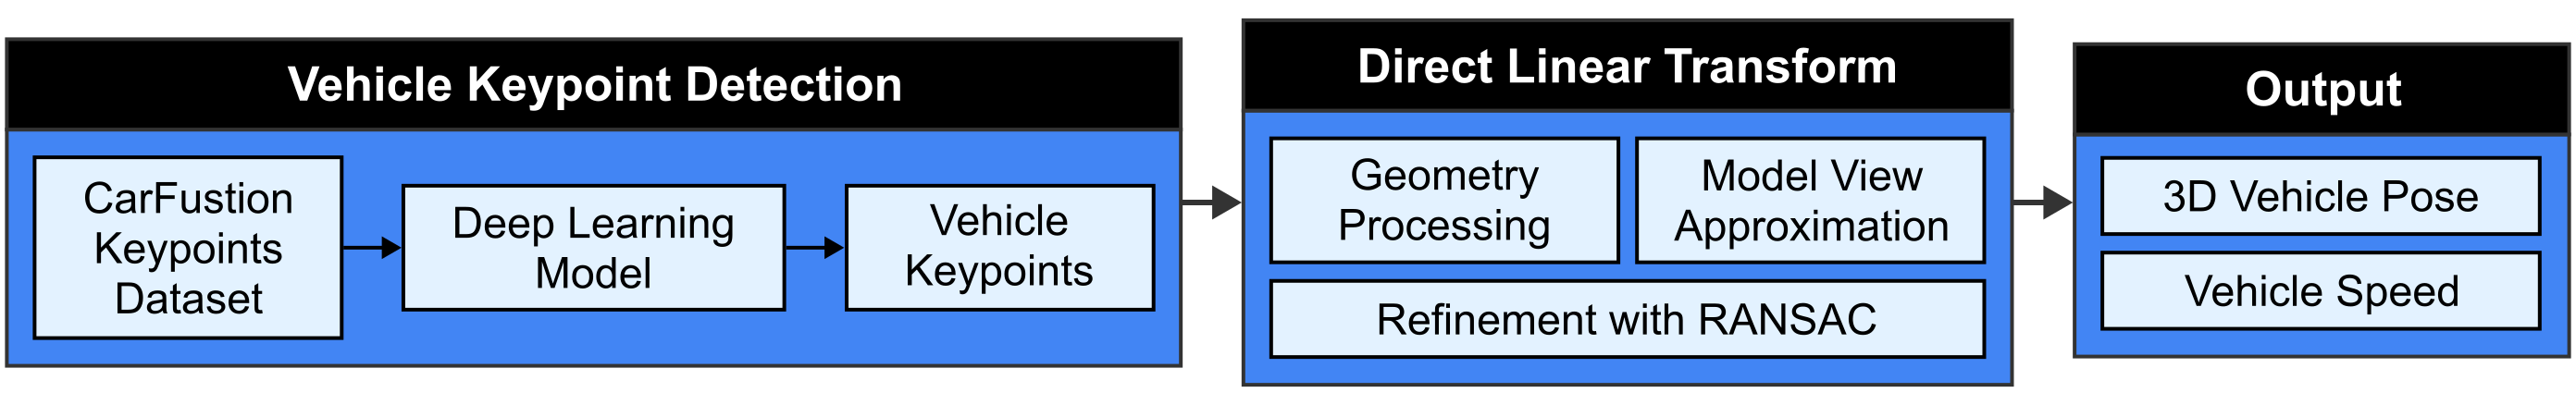
\includegraphics[width=1\columnwidth]{./images/workflow.png}
    \caption{Project workflow.}
    \label{img:workflow}
\end{figure}

\section{Vehicle Key Point Detection}

For this project, an adapted version of the OpenPifPaf pose-detection deep learning model for car keypoint detection was used, using Carfusion datasets for testing and training data \cite{CFusion}. The initial training was done with a pre-trained model with a ResNet-101 backbone. Then the model was trained on a subset of 10 images over 150 epochs. For this model the weight file as well as the keypoint data of the predicted image was successfully generated. 

\section{3D Pose Estimation}

\subsection{Geometry Processing}

To understand the 3d pose estimation process a basic understanding of the geometry processing stage of the 3d rendering pipeline is required. That is the process of how a 3d model and its vertices are transformed from points in 3d space to pixels on a 2d screen.

The vertices of a 3D model are defined in their local coordinate system, the so-called local space. If the model is placed inside the 3D scene, its position in world space can be controlled with the model matrix $M_{mod}$. World space is the coordinate system of the \textit{world}, the 3d scene where all the objects, lights, and the camera live. The camera's position and rotation in world space are determined by the inverse of the view matrix $M_{view}^{-1}$. For the next steps of the 3D rendering pipeline, it is generally preferred to have objects in view space rather than world space. View space is the reference frame of the camera, meaning the camera is located at its origin looking straight ahead. To transform an object from world- into viewspace, it just needs to be multiplied by the view matrix, meaning to get from local- to view space the composition of the model and view matrices can be used: this composition is called model view Matrix $M_{MV}=M_{view}M_{mod}$.

The next step is figuring out where on the screen a vertex should be drawn. Once in view space, the projected position on the $z = 1$ plane can be computed by dividing the position of a vertex by its z-component. More formally you can multiply by the projection matrix and divide by the w-component. This matrix representation of the standard projection onto the $z = 1$ plane looks like this:

\begin{equation}
    \begin{bmatrix}
        1 & 0 & 0 & 0 \\
        0 & 1 & 0 & 0 \\
        0 & 0 & 1 & 0 \\
        0 & 0 & 1 & 0
    \end{bmatrix}
    \begin{bmatrix}
        x \\
        y \\
        z \\
        1
    \end{bmatrix}
    =
    \begin{bmatrix}
        x \\
        y \\
        z \\
        z
    \end{bmatrix}
    \overset{\text{div z}}{\equiv}
    \begin{bmatrix}
        \frac{x}{z} \\
        \frac{y}{z} \\
        1           \\
    \end{bmatrix}
\end{equation}

The projection still needs to be modified to have more control over what exactly is seen on the screen. Instead of projecting on the $z=1$ plane, objects are projected onto the $z=n$ plane, the near plane. To preserve depth information objects are not completely projected onto the near plane, but instead to the space between the near- and far planes. This is done by multiplying with $M_{P'}$ before dividing by the w component. This has no implications for this project, since there exists no depth information in the detected keypoints. Additionally since it is easier to work in relative coordinates when faced with pictures of different sizes, the projected view coordinates are finally transformed into normalized device coordinates (NDC) by multiplying with $M_{P''}$ (see \ref{eqn:API_matrix}). Normalized device coordinates are a coordinate system around the origin with the bounds of $\left[-1, 1\right]$ for every axis. The relative pixel coordinates of a vertex can simply be read off the $x$ and $y$ positions of the points in NDC. To get the exact pixel positions these relations between NDC- and pixel coordinates can be used:  $x_p = ({x'}/{2} + 0.5) \cdot width$ and $y_p = ({y'}/{2} + 0.5) \cdot height$.

\begin{figure*}[h]
    \begin{equation} \label{eqn:API_matrix}
        M_{P} = M_{P''} M_{P'} =
        \begin{bmatrix}
            \frac{2}{r - l} & 0               & 0               & \frac{-(r + l)}{r - l} \\
            0               & \frac{2}{t - b} & 0               & \frac{-(t + b)}{t - b} \\
            0               & 0               & \frac{2}{f - n} & \frac{-(f + n)}{f - n} \\
            0               & 0               & 0               & 1
        \end{bmatrix}
        \begin{bmatrix}
            n & 0 & 0     & 0   \\
            0 & n & 0     & 0   \\
            0 & 0 & n + f & -nf \\
            0 & 0 & 1     & 0
        \end{bmatrix}
        =
        \begin{bmatrix}
            c_1 & 0   & 0   & 0   \\
            0   & c_2 & 0   & 0   \\
            0   & 0   & c_3 & c_4 \\
            0   & 0   & 1   & 0
        \end{bmatrix}
    \end{equation}
    \caption[]{The values $r$, $l$, $t$ and $b$ can be calculated from the focal length and sensor size of the camera (see \ref{img:fov}). E.g., $r$ can be calculated in the following way:
        $r = n \cdot \tan\left(\frac{FOV}{2}\right),
            FOV = 2 \cdot \arctan\left(\frac{s_w}{2f}\right)$,
        ($s_w$ = sensor width, $f$ = focal length, $FOV$ = field of view).
    }
\end{figure*}

\begin{figure}[H]
    \centering
    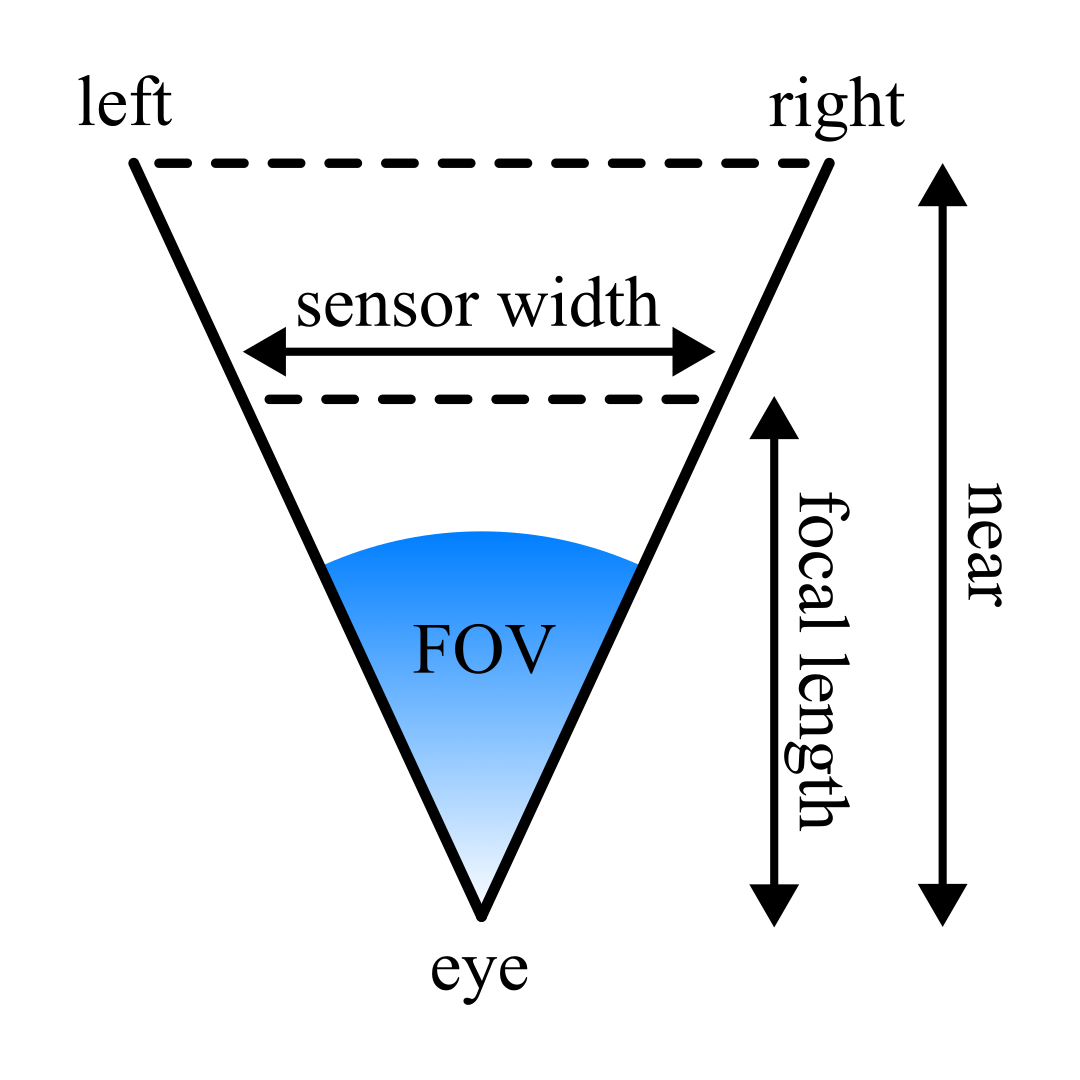
\includegraphics[width=0.4\columnwidth]{./images/focal_lenght_and_field_of_view.png}
    \caption{The sensor width and the focal length are used to calculate the camera's field of view.}
    \label{img:fov}
\end{figure}

This process basically transforms the view frustum into a cube of side length two around the origin (see \ref{img:view_to_ndc}).

\begin{figure}[H]
    \centering
    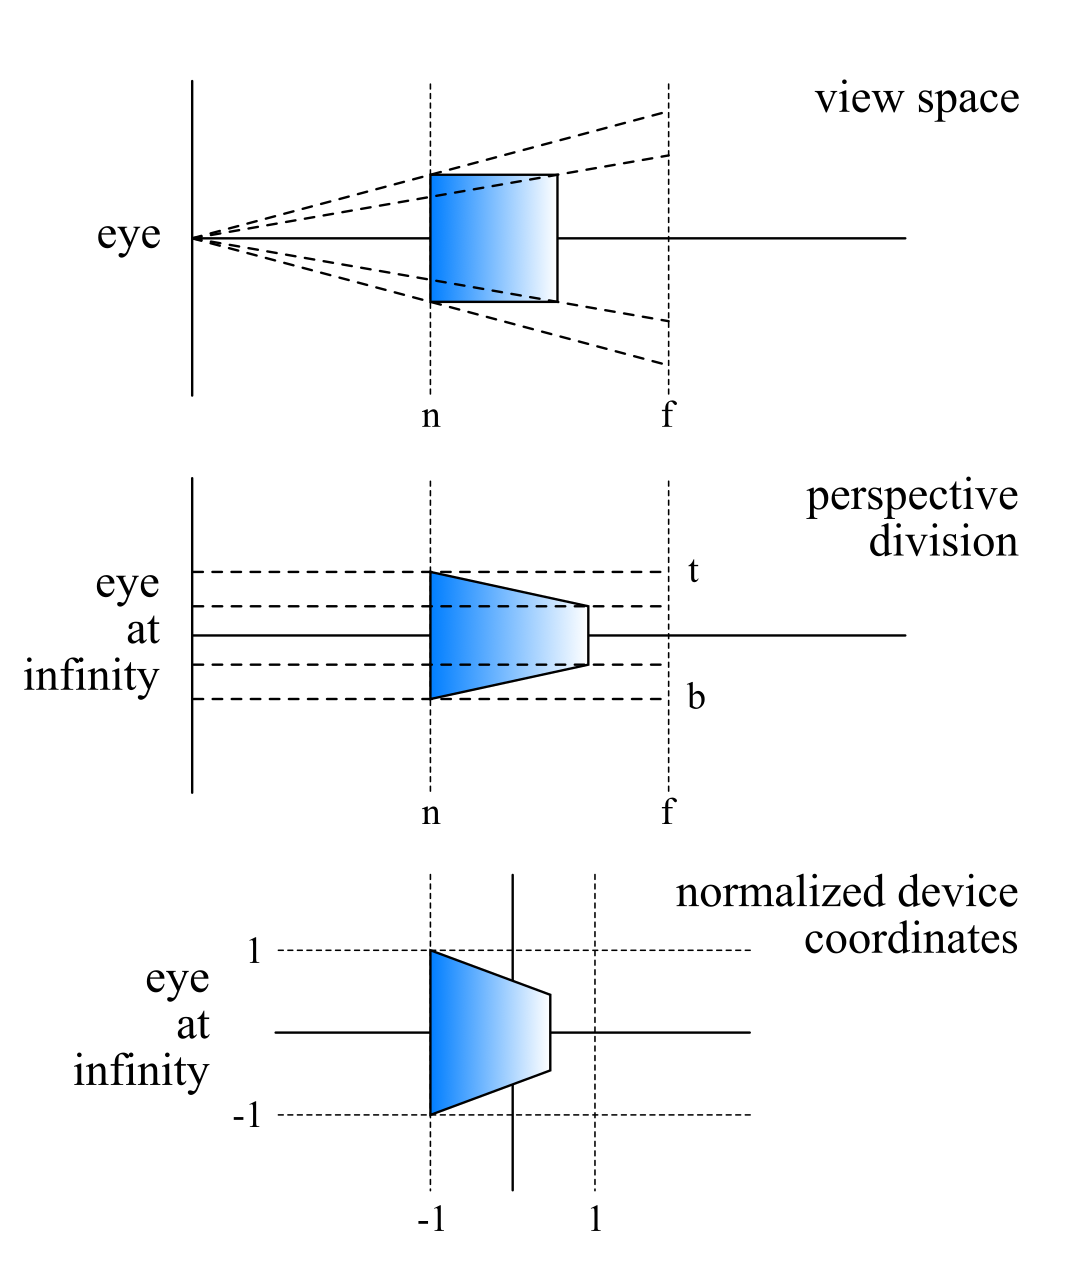
\includegraphics[width=0.8\columnwidth]{./images/view_coordinates_to_ndc.png}
    \caption{Perspective projection from view space to NDC in 2d.}
    \label{img:view_to_ndc}
\end{figure}

\subsection{Modelview Matrix Approximation}

To get the approximate 3d position of the cars, the detected 2d key points need to be correlated with their 3d counterparts. As discussed earlier the screen space positions can be computed by multiplying the vertices in local space with the modelview matrix $M_{MV}$ and the projection matrix $M_P$ before dividing by w.

\begin{equation}
    \begin{bmatrix}
        1 & 0 & 0 & 0 \\
        0 & 1 & 0 & 0 \\
        0 & 0 & 1 & 0 \\
        0 & 0 & 1 & 0
    \end{bmatrix}
    \begin{bmatrix}
        x \\
        y \\
        z \\
        1
    \end{bmatrix}
    =
    \begin{bmatrix}
        x \\
        y \\
        z \\
        z
    \end{bmatrix}
    \overset{\text{div z}}{\equiv}
    \begin{bmatrix}
        \frac{x}{z} \\
        \frac{y}{z} \\
        1           \\
    \end{bmatrix}
\end{equation}

This matrix multiplication and the final division by the homogeneous component can be performed and solved for $x'$ and $y'$ that gives:

\begin{equation}
    x' = \frac{c_1 a x + c_1 b y + c_1 c z + c_1 d}{ix + jy + kz + l}
\end{equation}
\begin{equation}
    y' = \frac{c_2 e x + c_2 f y + c_2 g z + c_2 h}{ix + jy + kz + l}
\end{equation}

Now one can multiply by the denominator and set both equations to 0. With the assumption that the focal length and sensor size of the camera are known and having a matching from the key points to the vertices of a 3d model, the only unknown are the values of $M_{MV}$, meaning $c_{1}..c_{4}$. Since this relation hold for every pair of points (($p_{1} , p_{1}'), (p_{2} , p_{2}'), ..., (p_{n}, p_{n}'$)), the following system of equation can be created (see \ref{eqn:DLT}).

\begin{figure*}[h]
    \begin{equation} \label{eqn:DLT}
        \begin{bmatrix}
            -c_1 x_1 & -c_1 y_1 & -c_1 z_1 & -c_1   & 0        & 0        & 0        & 0      & x_1 x_{1}' & y_1 x_{1}' & z_1 x_{1}' & x_{1}' \\
            0        & 0        & 0        & 0      & -c_2 x_1 & -c_2 y_1 & -c_2 z_1 & -c_2   & x_1 y_{1}' & y_1 y_{1}' & z_1 y_{1}' & y_{1}' \\
            \vdots   & \vdots   & \vdots   & \vdots & \vdots   & \vdots   & \vdots   & \vdots & \vdots     & \vdots     & \vdots     & \vdots \\
            -c_1 x_n & -c_1 y_n & -c_1 z_n & -c_1   & 0        & 0        & 0        & 0      & x_n x_{n}' & y_n x_{n}' & z_n x_{n}' & x_{n}' \\
            0        & 0        & 0        & 0      & -c_2 x_n & -c_2 y_n & -c_2 z_n & -c_2   & x_n y_{n}' & y_n y_{n}' & z_n y_{n}' & y_{n}' \\
        \end{bmatrix}
        \begin{bmatrix}
            a      \\
            b      \\
            \vdots \\
            k      \\
            l
        \end{bmatrix}
        =
        \begin{bmatrix}
            0      \\
            0      \\
            \vdots \\
            0      \\
            0
        \end{bmatrix}
    \end{equation}
\end{figure*}

The solution to this homogeneous system of equations ($Ab = 0$) can be obtained by finding the null space of the matrix $A$. The null space is the set of all vectors $b$ that satisfy $Ab = 0$. This set can be found with the help of a  singular value decomposition (SVD) that factorizes a matrix $A$ into a rotation, followed by a rescaling followed by another rotation ($A = U\Sigma V^{T}$) \cite{SVD}. In the SVD the formula $Ab = U\Sigma V^{T}b = 0$ implies $V^{T}b = 0$ since $U$ is invertible and has no nontrivial solutions for $Ub = 0$. Thus $V^{T}b$ must be a vector where only the rows corresponding to zero singular values contribute to the null space. The columns of $V$ that correspond to zero singular values in $\Sigma$ combined form a basis for the null space of $A$. In this way one solution for the system of equations can be found. Out of this solution the following matrix can be created:

\begin{equation}
    \renewcommand{\arraystretch}{1.5}
    \left[\begin{array}{@{}c:c@{}}
            R                        & t \\ \hdashline
            \begin{array}{@{}ccc@{}}
                0 & 0 & 0
            \end{array} & 1
        \end{array}\right]
\end{equation}

Here $R$ stands for a $3\times3$ matrix that holds the rotation and scaling part of the solution and $t$ for a vector of size 3 containing the translation. Together they do not uniquely define the modelview matrix, since this result is scale invariant. At this point the model cannot distinguish between a big object far away and a small object close by since their projections on the screen would look the same to the camera. But the fact that the scale is 1 solves this dilemma. This means that $R$ is orthogonal, meaning it has only rotational components, but no scaling. The correct $R$ can be calculated with another SVD, by just omitting $\Sigma$, which avoids any scaling; a new $R$ can be calculated this way: $R' = UV^{T}$. The last step is scaling $t$ by the same amount and replacing $R$ by $R'$ in the result; the modelview matrix is found.

For this process to work it is very important that the 3d model is as close as possible to the real geometry of the object where the key points came from. To minimize differences our model uses three different car wireframes \ref{img:wireframes} and picks the one with the smallest fitting error (the error is the sum of distances of the key points and projected 3d vertices in NDC). The different cars were picked to cover a wide range of possible car sizes, from midsized, over station wagons up to SUVs.

\begin{figure}[H]
    \centering
    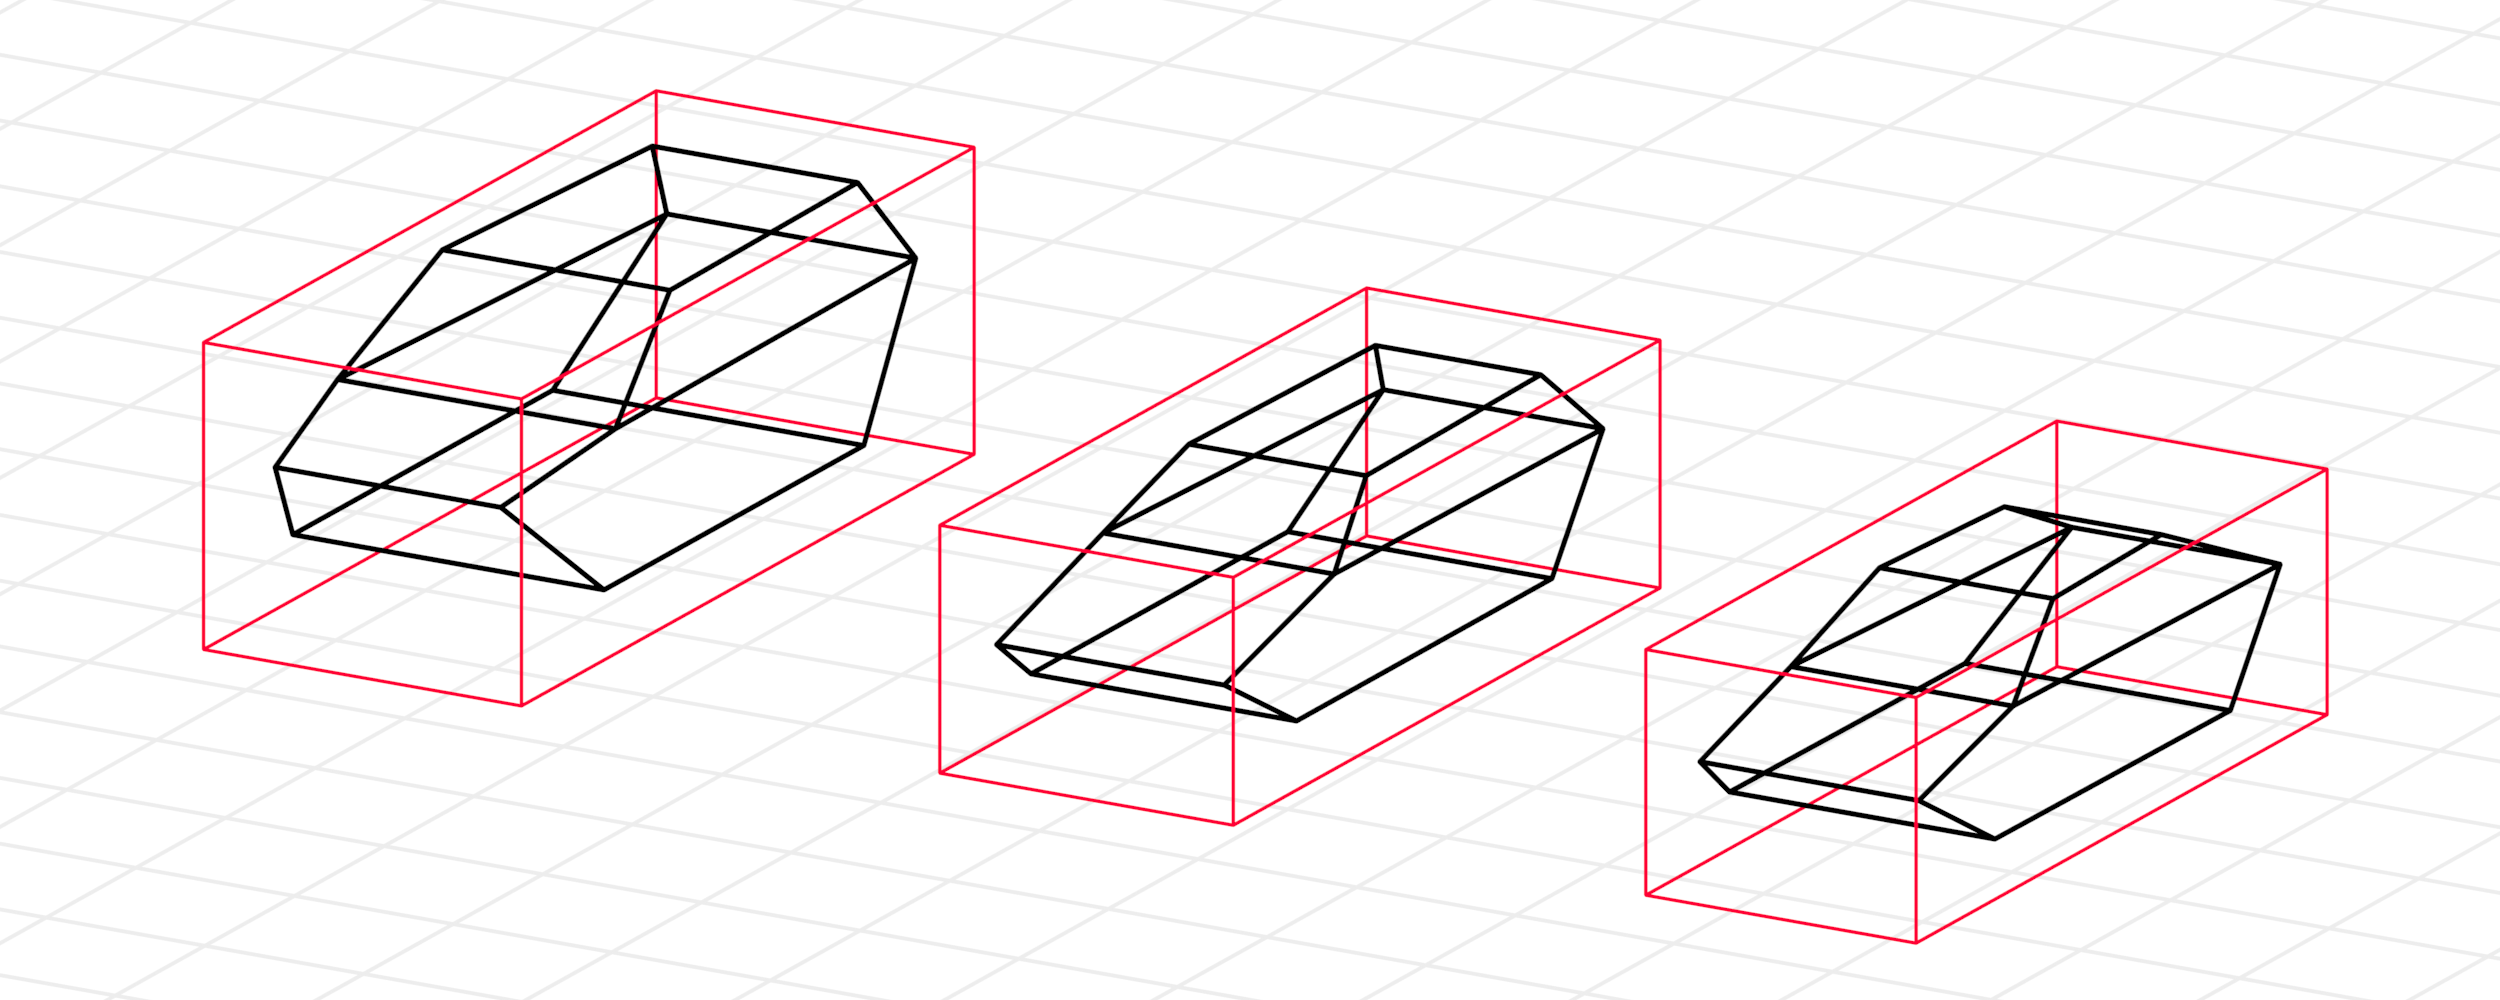
\includegraphics[width=0.7\columnwidth]{./images/wireframes.png}
    \caption{Different car wireframes used. From left to right Ford Explorer, Volvo V60, Nissan Altima.}
    \label{img:wireframes}
\end{figure}

\subsection{Estimation Refinement}

Since the detected key points can be incorrect it is of utmost importance that the model is robust against outliers and small errors. This problem can be improved by utilizing random sample consensus (RANSAC), an algorithm that estimates the right parameters for a mathematical model from a set of measured/observed data that can contain outliers or values with large errors \cite{RANSAC}. In this case the basic RANSAC algorithm has been modified slightly to check all subsets of a specific size, since the total number of samples is $\leq$ 14, meaning the total number of subsets is a manageable size. This transforms this version of RASAC into a deterministic algorithm that always produces the same output.

\section{Speed Estimation}

\subsection{Car Matching Over Multiple Frames}

To calculate the speed, it is not enough to know the relative location of the car at a specific point in time. It is also necessary to know the location of the same car at a different point in time. Since the Keypoint Detection step only detects the car's key points and bounding box, it is not trivial to know which car is which in the next frame. But since videos are usually shot at 30fps or more, a car's bounding box does not move very far from one frame to another. Considering this and the fact that generally there are not a lot of cars whose bounding boxes overlap, the simple approach of matching the two cars whose bounding boxes are closest to each other works just fine. To allow new cars to enter the frame and old cars to leave the frame the variable $max\_distance$ is used, which describes the maximum distance a car can move from one frame to the next.

\begin{lstlisting}[language=Python, basicstyle=\small, tabsize=4]
#Pseudo code of the matching process
#cars keeps track of all the cars in the scene
#cars_n contains all the cars in the new frame
for old_car in cars:
    c, d = closest_car(cars_n, old_car)
    if d > max_distance:
        #the car left the frame
        cars.remove(old_car)
    else:
        old.match(c)
        #every car can only be matched once
        cars_n.remove(new_car)

#all remaining not matched new cars
for new_car in cars_n: 
    #a new car has entered the frame 
    cars.append(new_car) 
\end{lstlisting}

Once the 3d position of a car over multiple frames is known, the car's speed can be calculated by dividing the distance traveled by the elapsed time.

\section{Experimental Results}

The key point detection model accurately detects the key points accurately in most situations as seen in \ref{img:keypoints}.

\begin{figure}[h]
    \centering
    \subfloat[\centering Example 1]{{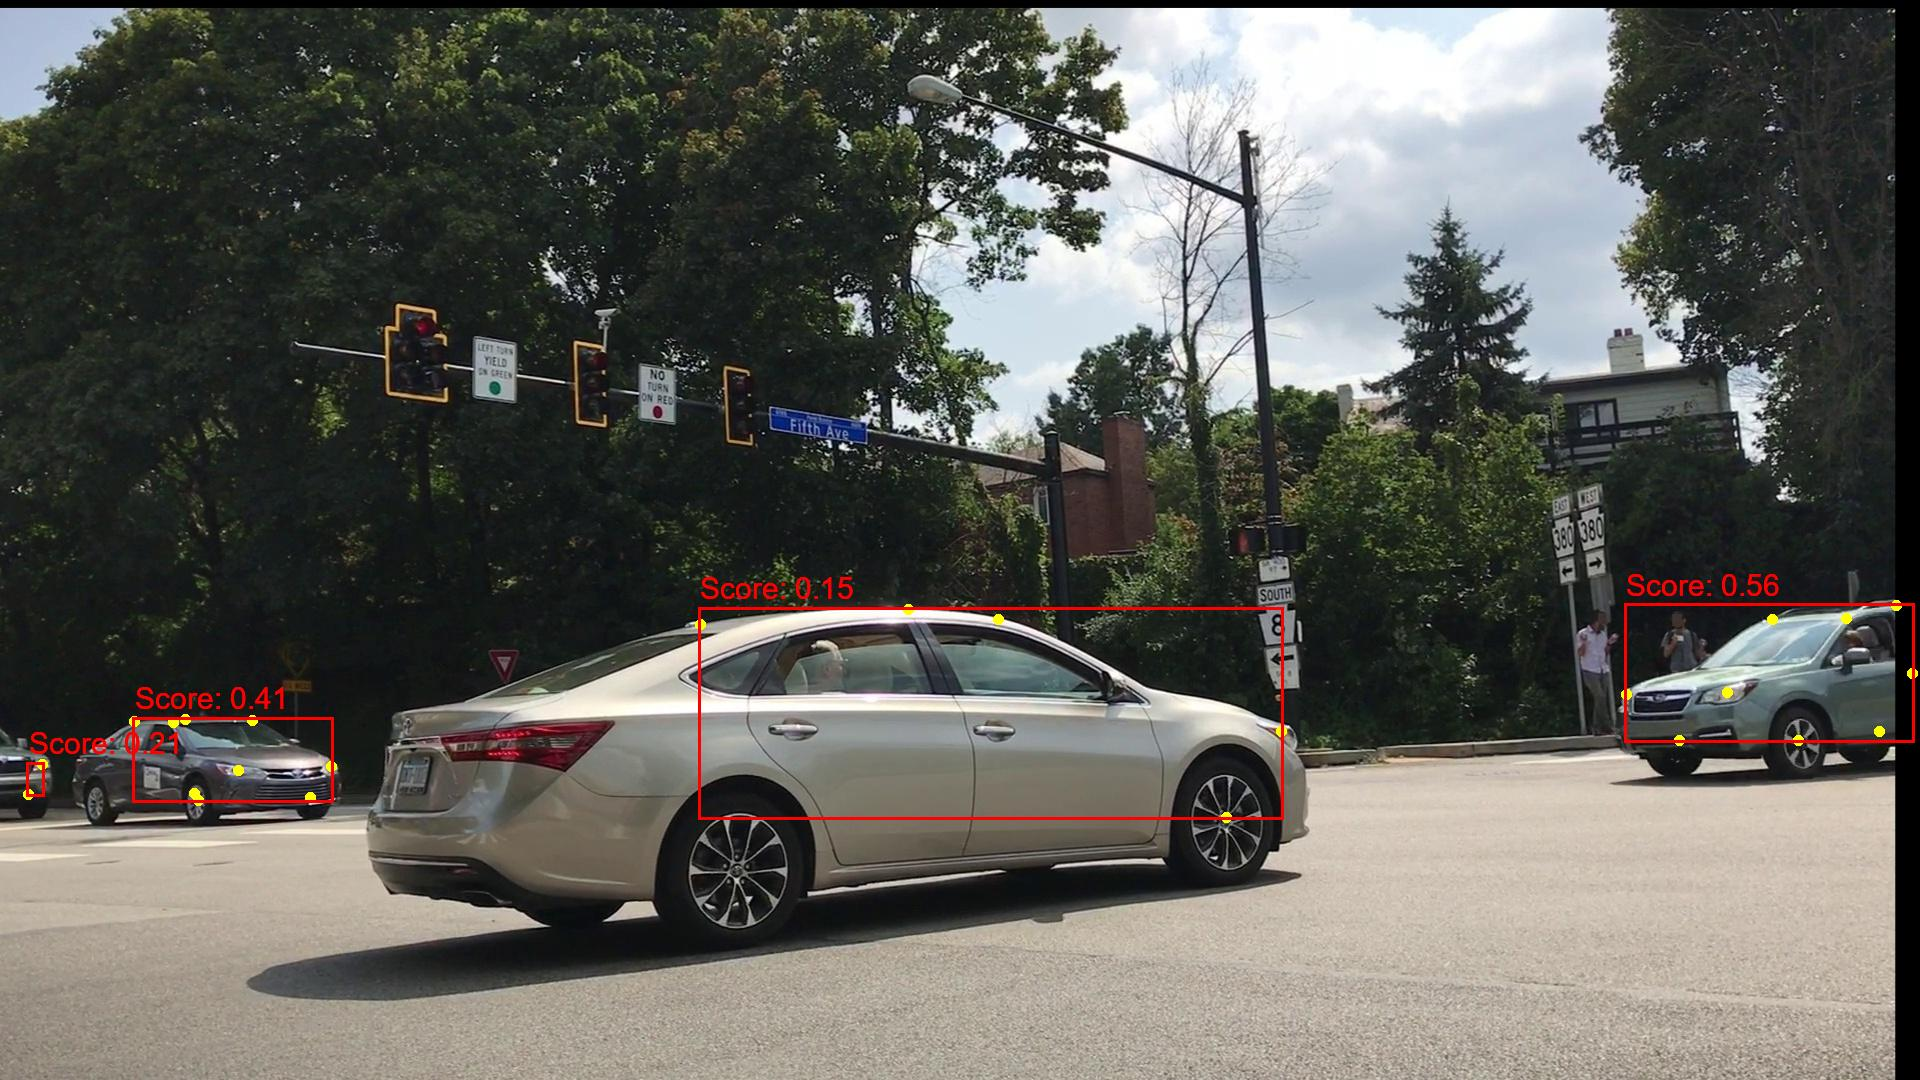
\includegraphics[width=.48\columnwidth]{./images/keypoint_vis1.jpg} }}
    \subfloat[\centering Example 2]{{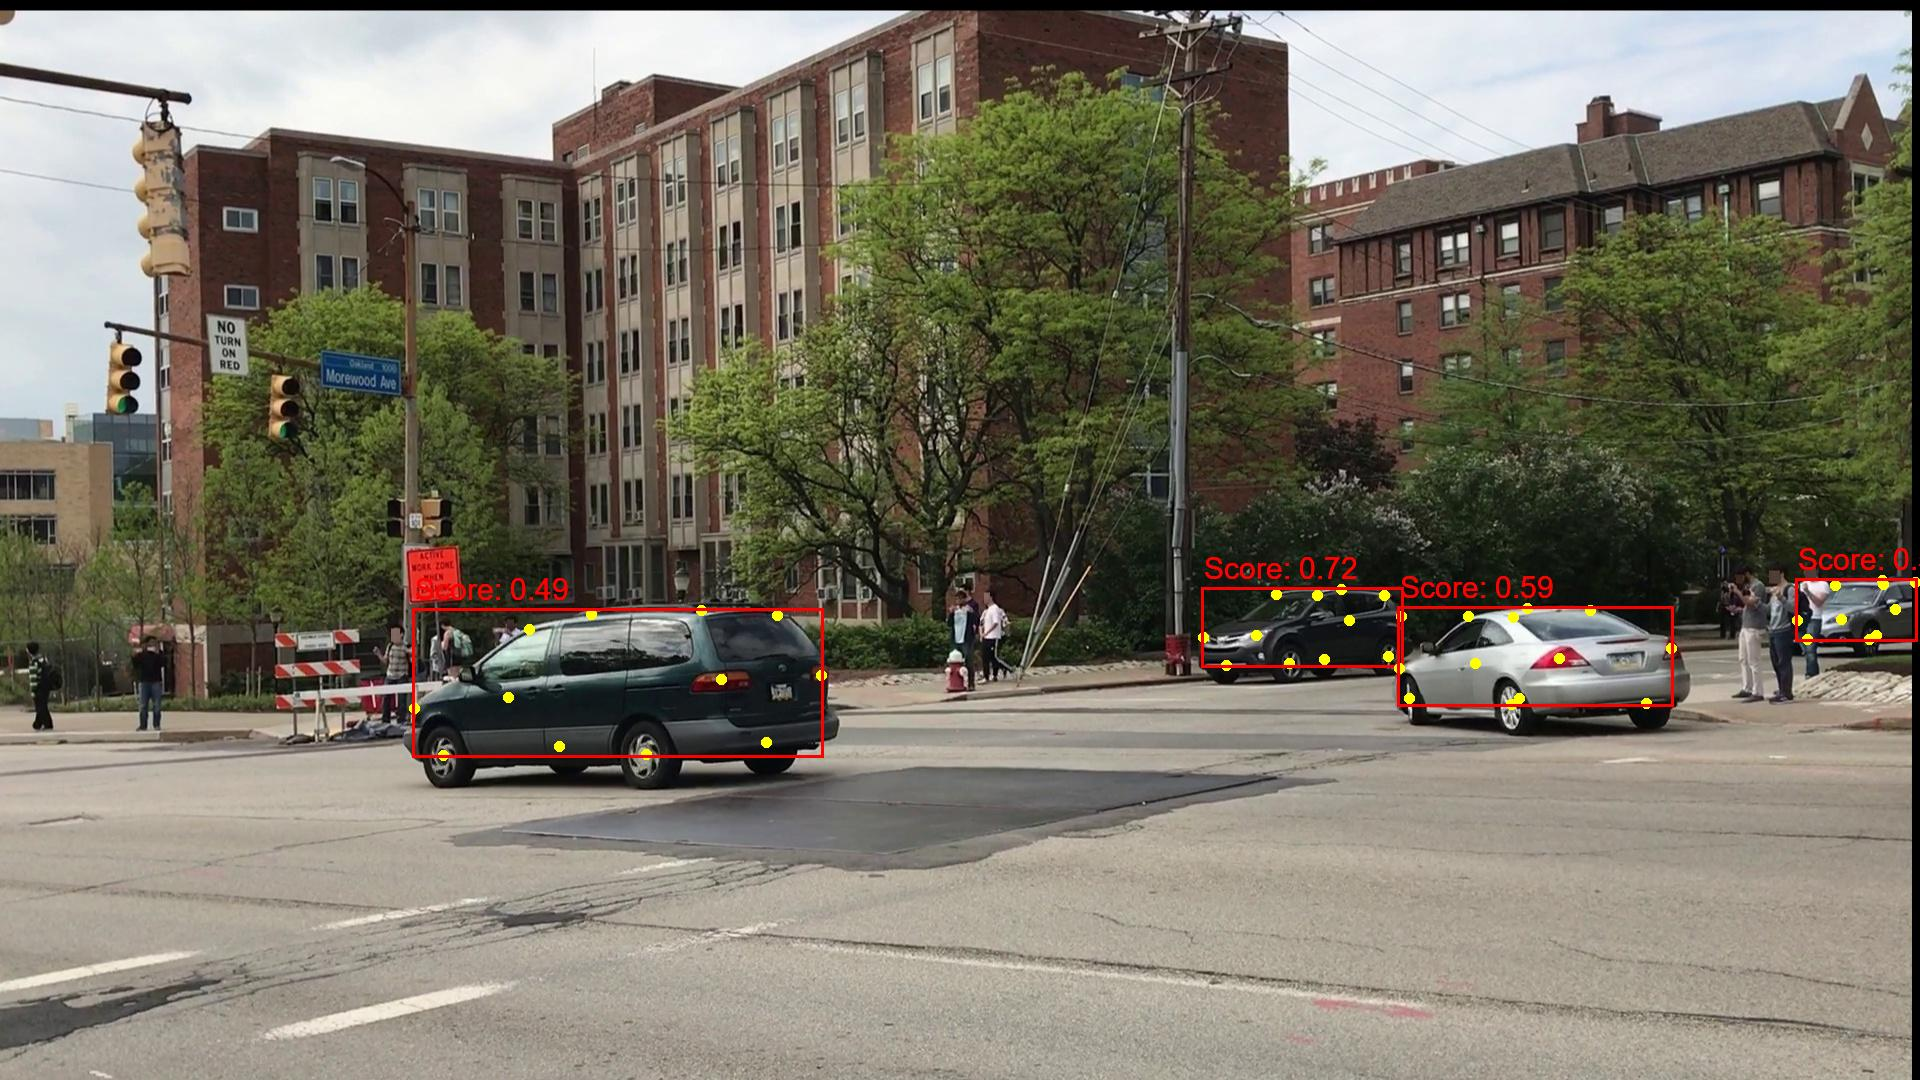
\includegraphics[width=.48\columnwidth]{./images/keypoint_vis3.jpg} }}
    \caption{Examples of the predicted key points from the OpenPifPaf model. Detected keypoints are shown in yellow and the computed bounding box in red. The overall confidence score is shown above the bounding box.}
    \label{img:keypoints}
\end{figure}

Results of the second part of the project are not as good. Figures \ref{img:good} and \ref{img:decent} show acceptable results, but this is unfortunately the exception and not the norm. While the 3d model is positioned in the right position for almost all images, the accuracy is not big enough to correctly approximate the speed of the vehicles as shown in \ref{img:incorrectSpeed} and \ref{img:incorrectModel}. An additional problem can be seen in \ref{img:incorrectModel} where the 3d pose of the Truck cannot be estimated reliably since the library of 3d models does not include a similar vehicle. 

\begin{figure}[htbp]
    \centering
    \subfloat[\centering Example 1]{{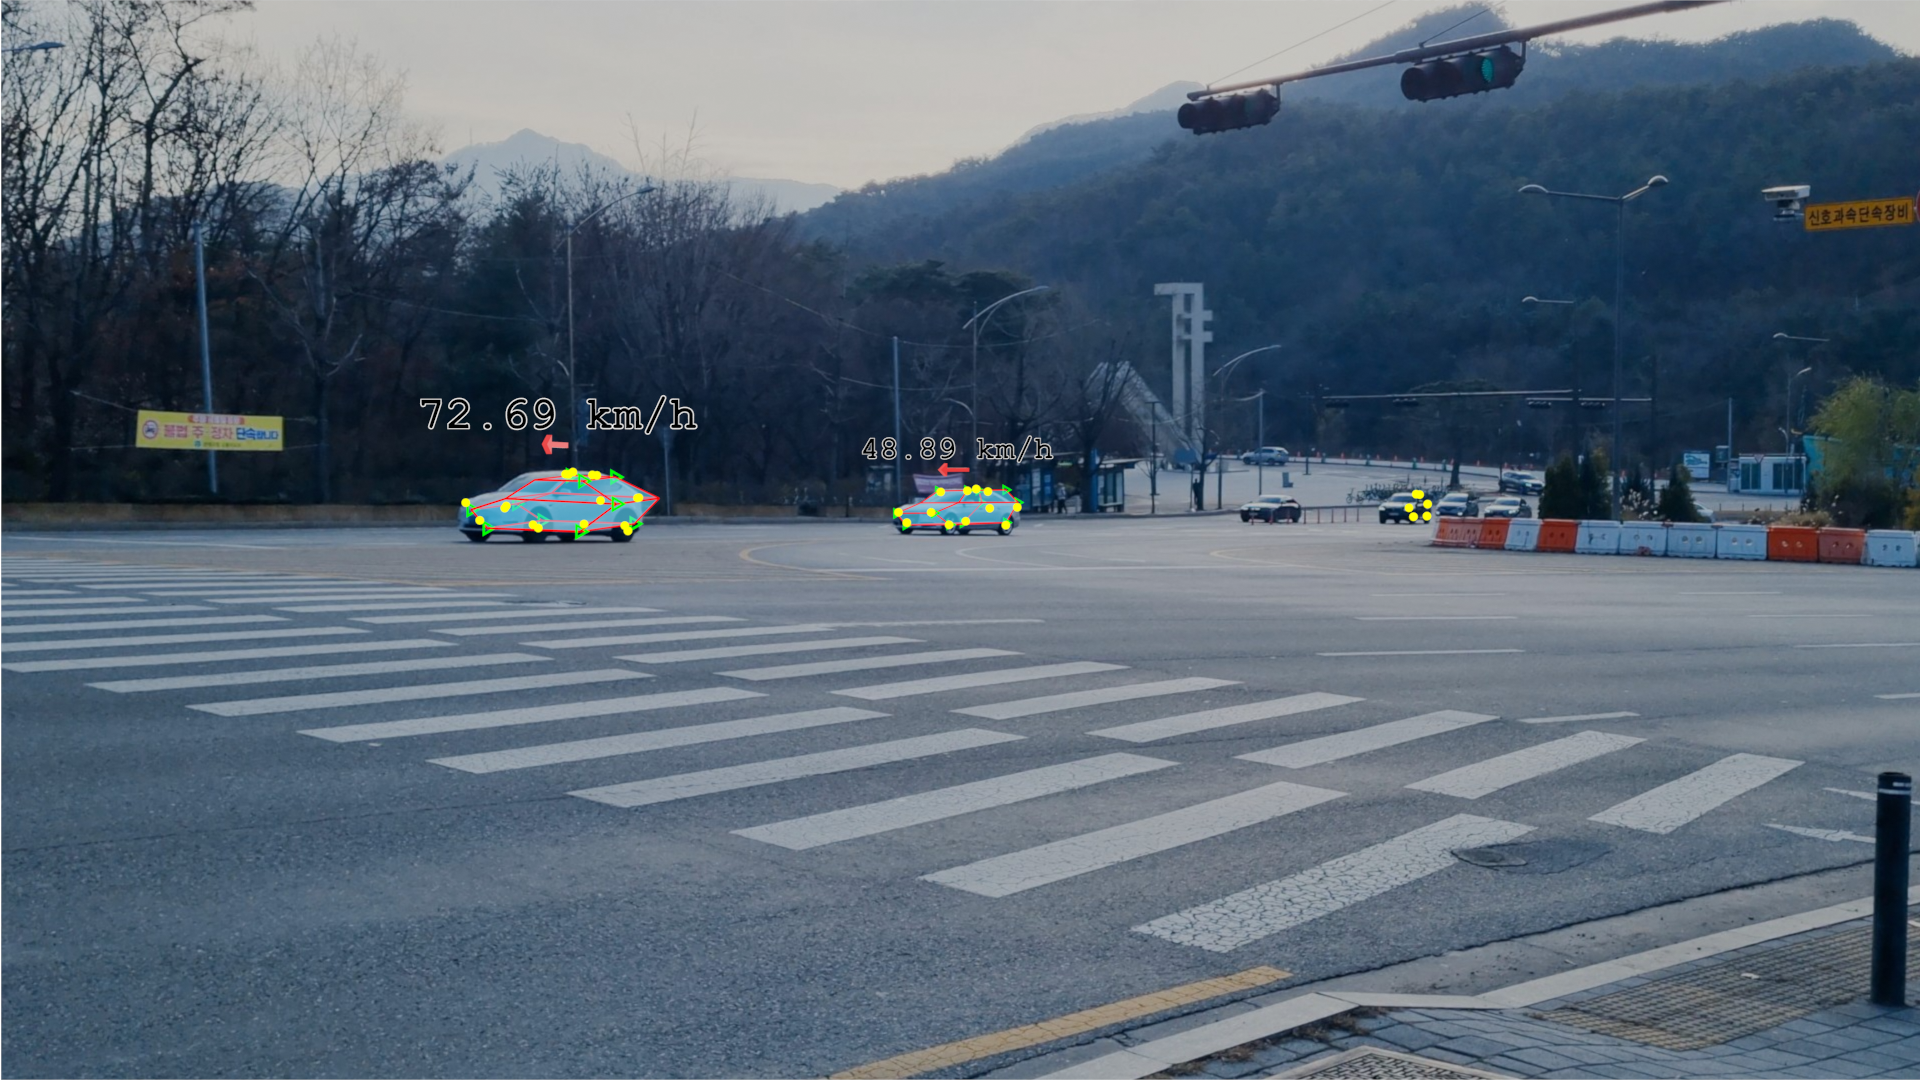
\includegraphics[width=.9\columnwidth]{./images/video5_out_1080.png}} \label{img:good}}
    \qquad
    \subfloat[\centering Example 2]{{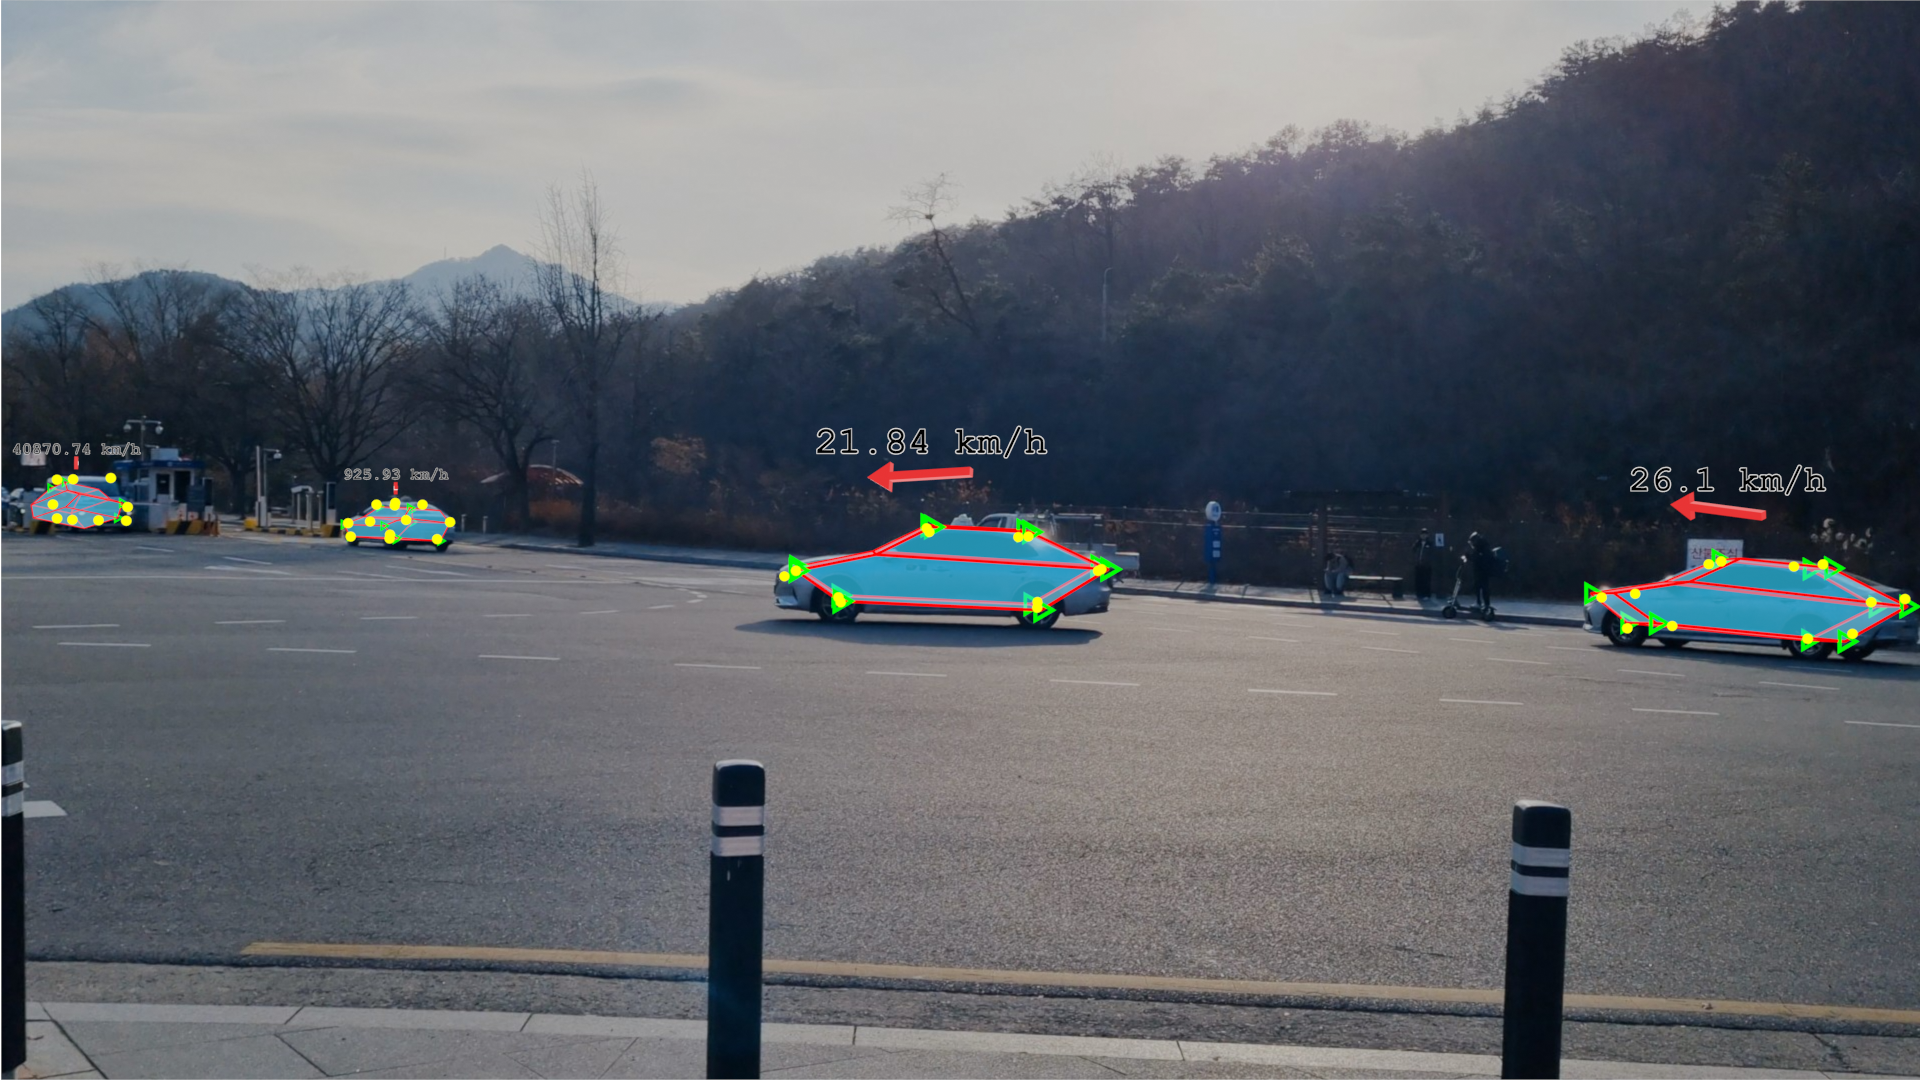
\includegraphics[width=.9\columnwidth]{./images/custom_0155.png} } \label{img:decent}}
    \qquad
    \subfloat[\centering Example 3]{{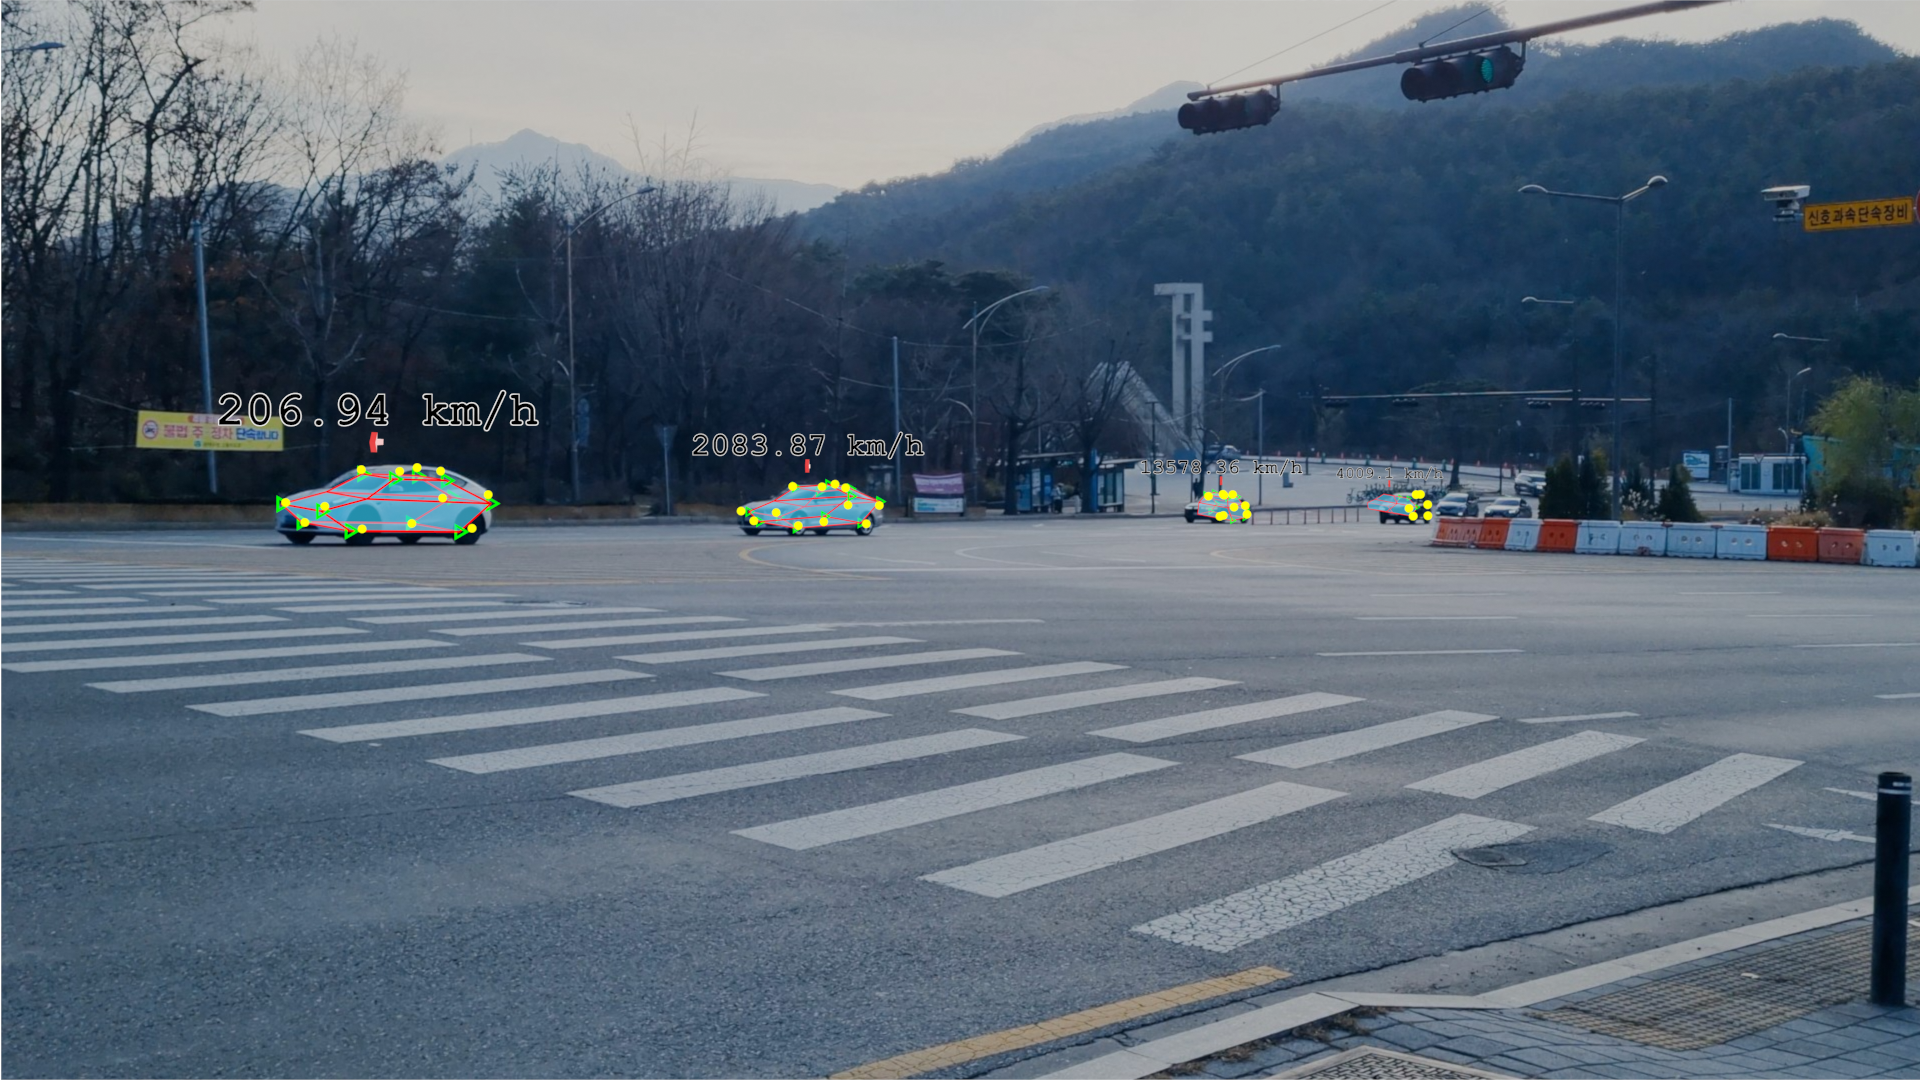
\includegraphics[width=.9\columnwidth]{./images/video5_out_1096.png} } \label{img:incorrectSpeed}}
    \qquad
    \subfloat[\centering Example 4]{{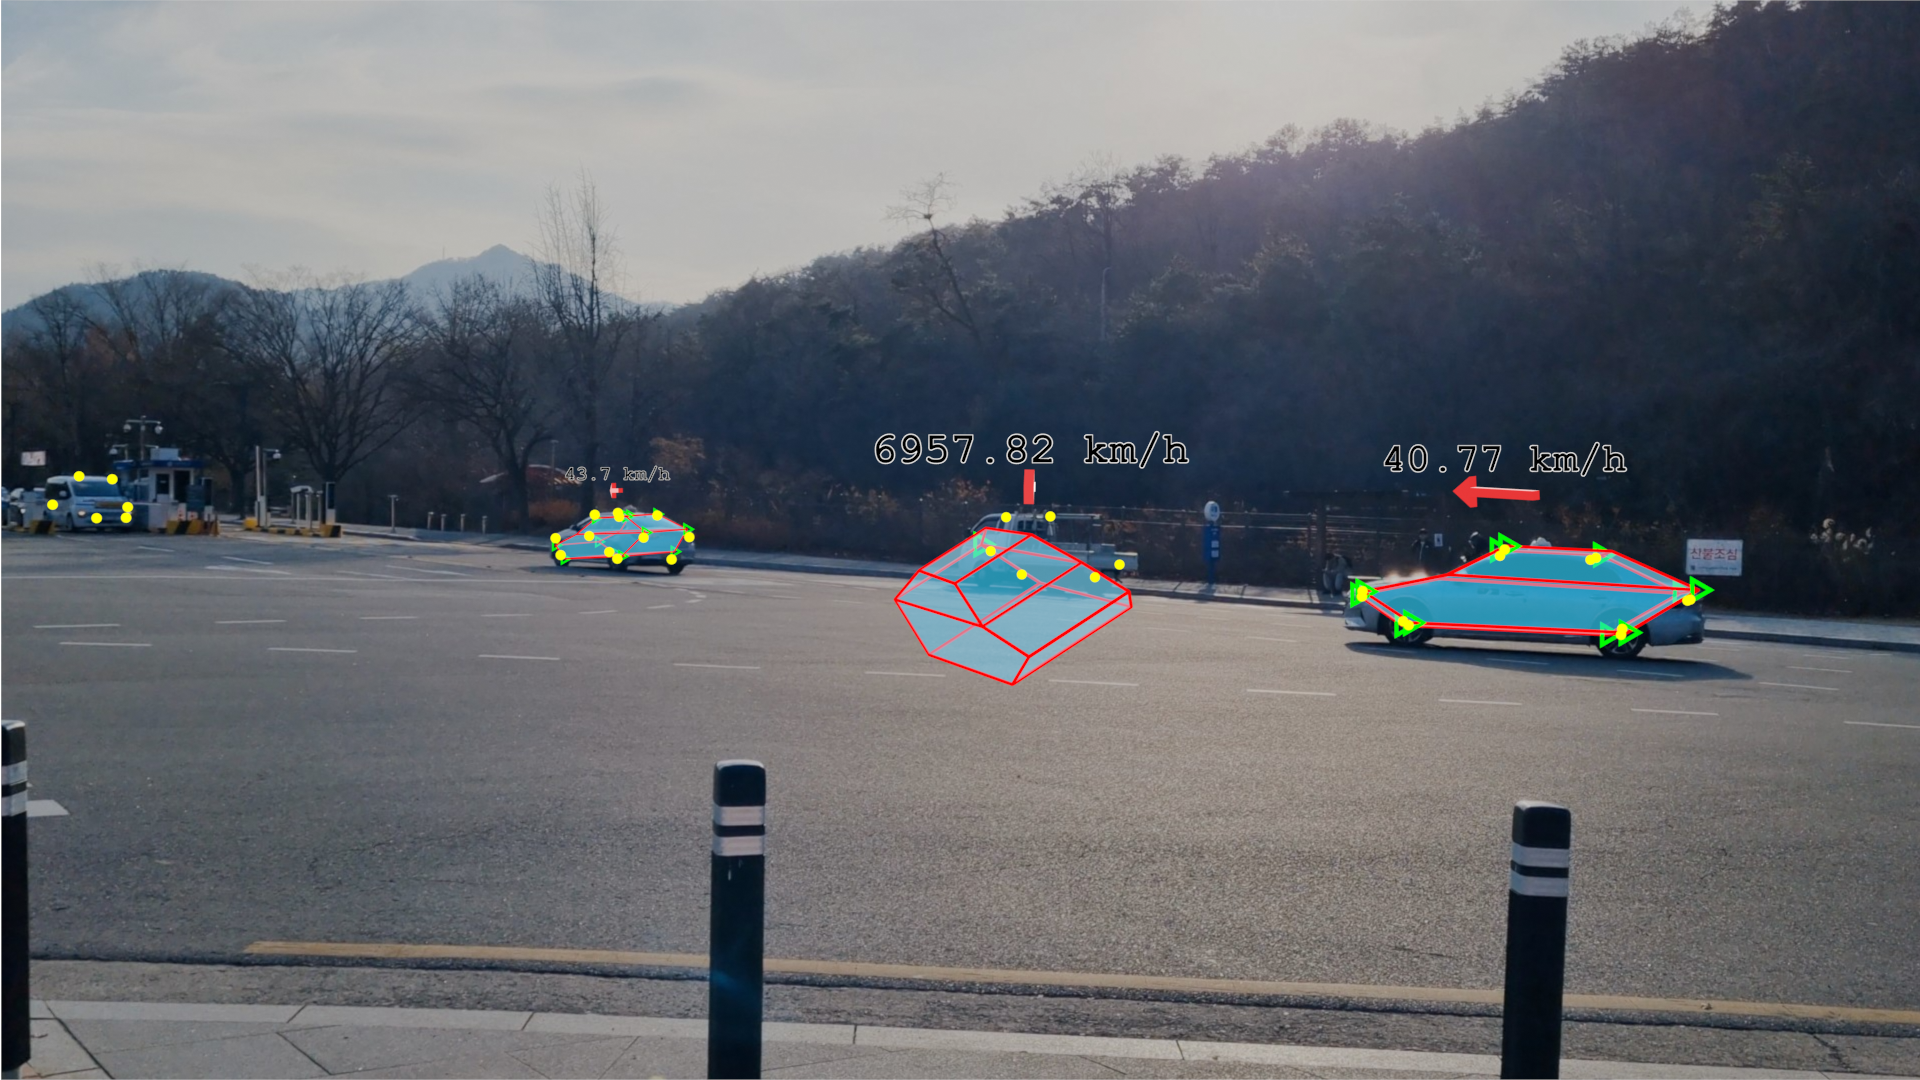
\includegraphics[width=.9\columnwidth]{./images/custom_0116.png} } \label{img:incorrectModel}}
    \caption{Examples of the output of the direct linear transformation model. The detected keypoints are shown in yellow, the wireframe of the predicted 3d model in red. Inliers of the RANSAC model are shown with green triangles. The speed and its direction is shown above the respective car.}
    \label{img:exampleOutput}
\end{figure}

\section{Result Discussion}

Our project successfully outputs the general wireframe 3D vehicles with only monocular camera images input, while using deep learning only for keypoint detection and utilizing traditional computer vision algorithms, as shown in the previous part. In addition, we try to estimate the speed of vehicles through frame-by-frame tracking.

The project, while qualitatively effective in addressing the 3D vehicle pose estimation problem, has limitations that affect its precision and applicability. The Direct Linear Transformation (DLT) model heavily relies on the accuracy of detected keypoints and the fit between 2D and 3D models, which makes it less robust in scenarios with noisy or inconsistent keypoints. Though it produces convincing results for still consequent images, it produces less optimal results for image sequences when speed calculation was performed. Additionally, our proposed method struggles with maintaining accuracy over image sequences, especially for dynamic tasks like vehicle speed calculation, and lacks sophisticated or robust tracking mechanisms for occluded objects with overlapping bounding boxes. 

Another problem is that while utilizing deep learning models only for the first step, the model still takes multiple seconds per frame for its computations, which is still not appropriate for real-time applications.

\subsection{Possible Improvements}

The direct linear transformation applied on image sequences was less accurate than initially hoped leading to good results for still images but less than optimal results for image sequences where the speed calculation was performed. Since the speed is calculated every frame only based on the current and previous positions the calculation is very susceptible to small errors. To help alleviate that problem some kind of temporal smoothing should be implemented. 

This would of course not be a problem if the estimated 3d pose was accurate. To achieve better results without completely overhauling the entire algorithm, a larger library of possible car models could be used to have a better matching between 2d key points and 3d vertices. This could be a big improvement since the direct linear transformation model basically delivers perfect results for good key points where the underlying 3d model is known.

Another area of improvement is the tracking of cars over multiple frames. In its current status it is very primitive and not robust against overlapping bounding boxes. Possible improvements include an implementation of the Kalman filter to better predict the next possible position.

\section{Materials}

The original source code for the keypoint detection can be found here \cite{keypoints} and the source code for the 3d pose reconstruction and 3d visualization is available on this github repository \cite{keypoint2pose}.

\section{Conclusion}

In this project, we developed a framework for wireframe 3D vehicle reconstruction from monocular camera input, combining deep learning for keypoint detection in the initial stage with traditional computer vision algorithms, including Direct Linear Transformation, for subsequent pose estimation. In addition, we extended our project to estimate vehicle speed using frame-by-frame tracking of 3D positions of vehicles. Our approach focuses on leveraging the efficiency and interpretability of geometry-based methods while minimizing the computational overhead typically associated with deep learning models.

The qualitative results demonstrate that our framework effectively constructs approximate 3D vehicle models from monocular images, highlighting its potential for applications in scenarios where depth information from stereo cameras or LiDAR is unavailable. Despite these achievements, the system has limitations in precision, particularly when high accuracy is needed such as in estimating speed, and struggels when dealing with mismatches between 2D keypoints and 3D vehicle models or overlapping objects in dynamic scenes. These limitations, alongside the computational time required per frame, constrain its utility for real-time applications and more complex tracking tasks. While the current framework provides a strong foundation, we hope that future research will significantly expand its applicability and reliability in real-world scenarios.

\bibliographystyle{./IEEEtran.bst}
\bibliography{./robot_vision}

\end{document}
